% Options for packages loaded elsewhere
\PassOptionsToPackage{unicode}{hyperref}
\PassOptionsToPackage{hyphens}{url}
%
\documentclass[
]{article}
\usepackage{amsmath,amssymb}
\usepackage{lmodern}
\usepackage{iftex}
\ifPDFTeX
  \usepackage[T1]{fontenc}
  \usepackage[utf8]{inputenc}
  \usepackage{textcomp} % provide euro and other symbols
\else % if luatex or xetex
  \usepackage{unicode-math}
  \defaultfontfeatures{Scale=MatchLowercase}
  \defaultfontfeatures[\rmfamily]{Ligatures=TeX,Scale=1}
\fi
% Use upquote if available, for straight quotes in verbatim environments
\IfFileExists{upquote.sty}{\usepackage{upquote}}{}
\IfFileExists{microtype.sty}{% use microtype if available
  \usepackage[]{microtype}
  \UseMicrotypeSet[protrusion]{basicmath} % disable protrusion for tt fonts
}{}
\makeatletter
\@ifundefined{KOMAClassName}{% if non-KOMA class
  \IfFileExists{parskip.sty}{%
    \usepackage{parskip}
  }{% else
    \setlength{\parindent}{0pt}
    \setlength{\parskip}{6pt plus 2pt minus 1pt}}
}{% if KOMA class
  \KOMAoptions{parskip=half}}
\makeatother
\usepackage{xcolor}
\IfFileExists{xurl.sty}{\usepackage{xurl}}{} % add URL line breaks if available
\IfFileExists{bookmark.sty}{\usepackage{bookmark}}{\usepackage{hyperref}}
\hypersetup{
  pdftitle={CHIC599 Project 2},
  pdfauthor={36075596},
  hidelinks,
  pdfcreator={LaTeX via pandoc}}
\urlstyle{same} % disable monospaced font for URLs
\usepackage[margin=1in]{geometry}
\usepackage{longtable,booktabs,array}
\usepackage{calc} % for calculating minipage widths
% Correct order of tables after \paragraph or \subparagraph
\usepackage{etoolbox}
\makeatletter
\patchcmd\longtable{\par}{\if@noskipsec\mbox{}\fi\par}{}{}
\makeatother
% Allow footnotes in longtable head/foot
\IfFileExists{footnotehyper.sty}{\usepackage{footnotehyper}}{\usepackage{footnote}}
\makesavenoteenv{longtable}
\usepackage{graphicx}
\makeatletter
\def\maxwidth{\ifdim\Gin@nat@width>\linewidth\linewidth\else\Gin@nat@width\fi}
\def\maxheight{\ifdim\Gin@nat@height>\textheight\textheight\else\Gin@nat@height\fi}
\makeatother
% Scale images if necessary, so that they will not overflow the page
% margins by default, and it is still possible to overwrite the defaults
% using explicit options in \includegraphics[width, height, ...]{}
\setkeys{Gin}{width=\maxwidth,height=\maxheight,keepaspectratio}
% Set default figure placement to htbp
\makeatletter
\def\fps@figure{htbp}
\makeatother
\setlength{\emergencystretch}{3em} % prevent overfull lines
\providecommand{\tightlist}{%
  \setlength{\itemsep}{0pt}\setlength{\parskip}{0pt}}
\setcounter{secnumdepth}{-\maxdimen} % remove section numbering
\newlength{\cslhangindent}
\setlength{\cslhangindent}{1.5em}
\newlength{\csllabelwidth}
\setlength{\csllabelwidth}{3em}
\newlength{\cslentryspacingunit} % times entry-spacing
\setlength{\cslentryspacingunit}{\parskip}
\newenvironment{CSLReferences}[2] % #1 hanging-ident, #2 entry spacing
 {% don't indent paragraphs
  \setlength{\parindent}{0pt}
  % turn on hanging indent if param 1 is 1
  \ifodd #1
  \let\oldpar\par
  \def\par{\hangindent=\cslhangindent\oldpar}
  \fi
  % set entry spacing
  \setlength{\parskip}{#2\cslentryspacingunit}
 }%
 {}
\usepackage{calc}
\newcommand{\CSLBlock}[1]{#1\hfill\break}
\newcommand{\CSLLeftMargin}[1]{\parbox[t]{\csllabelwidth}{#1}}
\newcommand{\CSLRightInline}[1]{\parbox[t]{\linewidth - \csllabelwidth}{#1}\break}
\newcommand{\CSLIndent}[1]{\hspace{\cslhangindent}#1}
\ifLuaTeX
  \usepackage{selnolig}  % disable illegal ligatures
\fi

\title{CHIC599 Project 2}
\author{36075596}
\date{2022-06-14}

\begin{document}
\maketitle

\hypertarget{introduction}{%
\subsection{Introduction}\label{introduction}}

Soil-transmitted helminthiases (STH) represents the highest burden of
disease for all neglected tropical diseases (NTD's) across the world
{[}\protect\hyperlink{ref-worldhealthorganizationEliminatingSoiltransmittedHelminthiases2012}{1}{]}.
The disease is caused mainly by three types of helminths: hookworms
(\emph{Necator americanus} and \emph{Ancylostoma duodenale}),
\emph{Ascaris lumbricoides} and \emph{Trichuris trichuria}. Although
they do not have high mortality rates, infections can have significant
impacts on health and quality of life. They are associated with stunted
growth, reduced cognitive development and micro-nutrient deficiency.
These effects are particularly concerning in school-age children and
pregnant women.

In Ethiopia, STH is a major public health concern, affecting over 79
million individuals
{[}\protect\hyperlink{ref-sartoriusPrevalenceIntensitySoiltransmitted2021}{2},\protect\hyperlink{ref-aemiroPrevalenceSoilTransmittedHelminthes2022}{3}{]}.
Following guidance from the World Health Organization (WHO), the
Ethiopian government launched a mass drug administration (MDA) project
in 2015. WHO recommends different MDA frequencies depending on the
prevalence of STH
{[}\protect\hyperlink{ref-worldhealthorganizationEliminatingSoiltransmittedHelminthiases2012}{1}{]}.
If prevalence is over 50\%, MDAs should take place twice a year. If
prevalence is between 20\% and 50\%, MDA should happen once a year. Any
areas where prevalence is under 20\% should change strategies and focus
on a case-by-case treatment schedule.

In this project, I used open-access data to predict the prevalence of
any STH across Ethiopia. I also produced probabilities of exceeding 50\%
prevalence and of falling between 20\% and 50\% prevalence. Using these
maps, I created discrete rasters identifying areas that required
treatment twice a year, areas that required treatment once a year, areas
that should move to a case-by-case strategy and areas for which the
uncertainty was too high to determine in which category they fell and
therefore would require further data collection.

\hypertarget{methods}{%
\section{Methods}\label{methods}}

\hypertarget{data-sources}{%
\subsection{Data sources}\label{data-sources}}

I downloaded STH data for Ethiopia from the Expanded Special Project to
Eliminate NTDs (ESPEN), a project set up by the WHO African Regional
Office to support national NTD control projects
{[}\protect\hyperlink{ref-ESPENExpandedSpecial}{4}{]}. The data set
contained geo-referrenced school surveys carried out across the country,
including the number of children examined and the number of children
that tested positive for each of the three STH groups (hookworms,
\emph{Ascaris lumbricoides} and \emph{Trichuris trichuria}). Each entry
had a geo-reliability and quality classification, referring to the
reliability of the recorded latitude and longitude and the quality of
the data. In my analyses, I only included those entries that had a
reliable location recorded and were of sufficient quality.

I used previous research to decide which covariates to download
{[}\protect\hyperlink{ref-alelignSoilTransmittedHelminthInfections2015}{5}--\protect\hyperlink{ref-eyayuPrevalenceIntensityInfection2022}{7}{]}.
These included elevation, sourced from
\href{https://www.diva-gis.org/}{DIVA GIS}
{[}\protect\hyperlink{ref-DIVAGISFreeSimple}{8}{]}, friction surface and
time to nearest healthcare centre, downloaded from the
\href{https://malariaatlas.org/}{Malaria Atlas Project}
{[}\protect\hyperlink{ref-MalariaAtlasProject}{9}{]} (Figure 1).
Friction surface estimates the minutes required to travel one meter over
land, producing a walking-only raster and a motorized vehicle raster.
Similarly, the time to nearest healthcare centre estimates the minutes
required to reach said centre, both walking-only and with motorized
vehicle. I also downloaded a shapefile of all the rivers in Ethiopia
which I used to create a raster of distance to the nearest river.

\begin{figure}
\centering
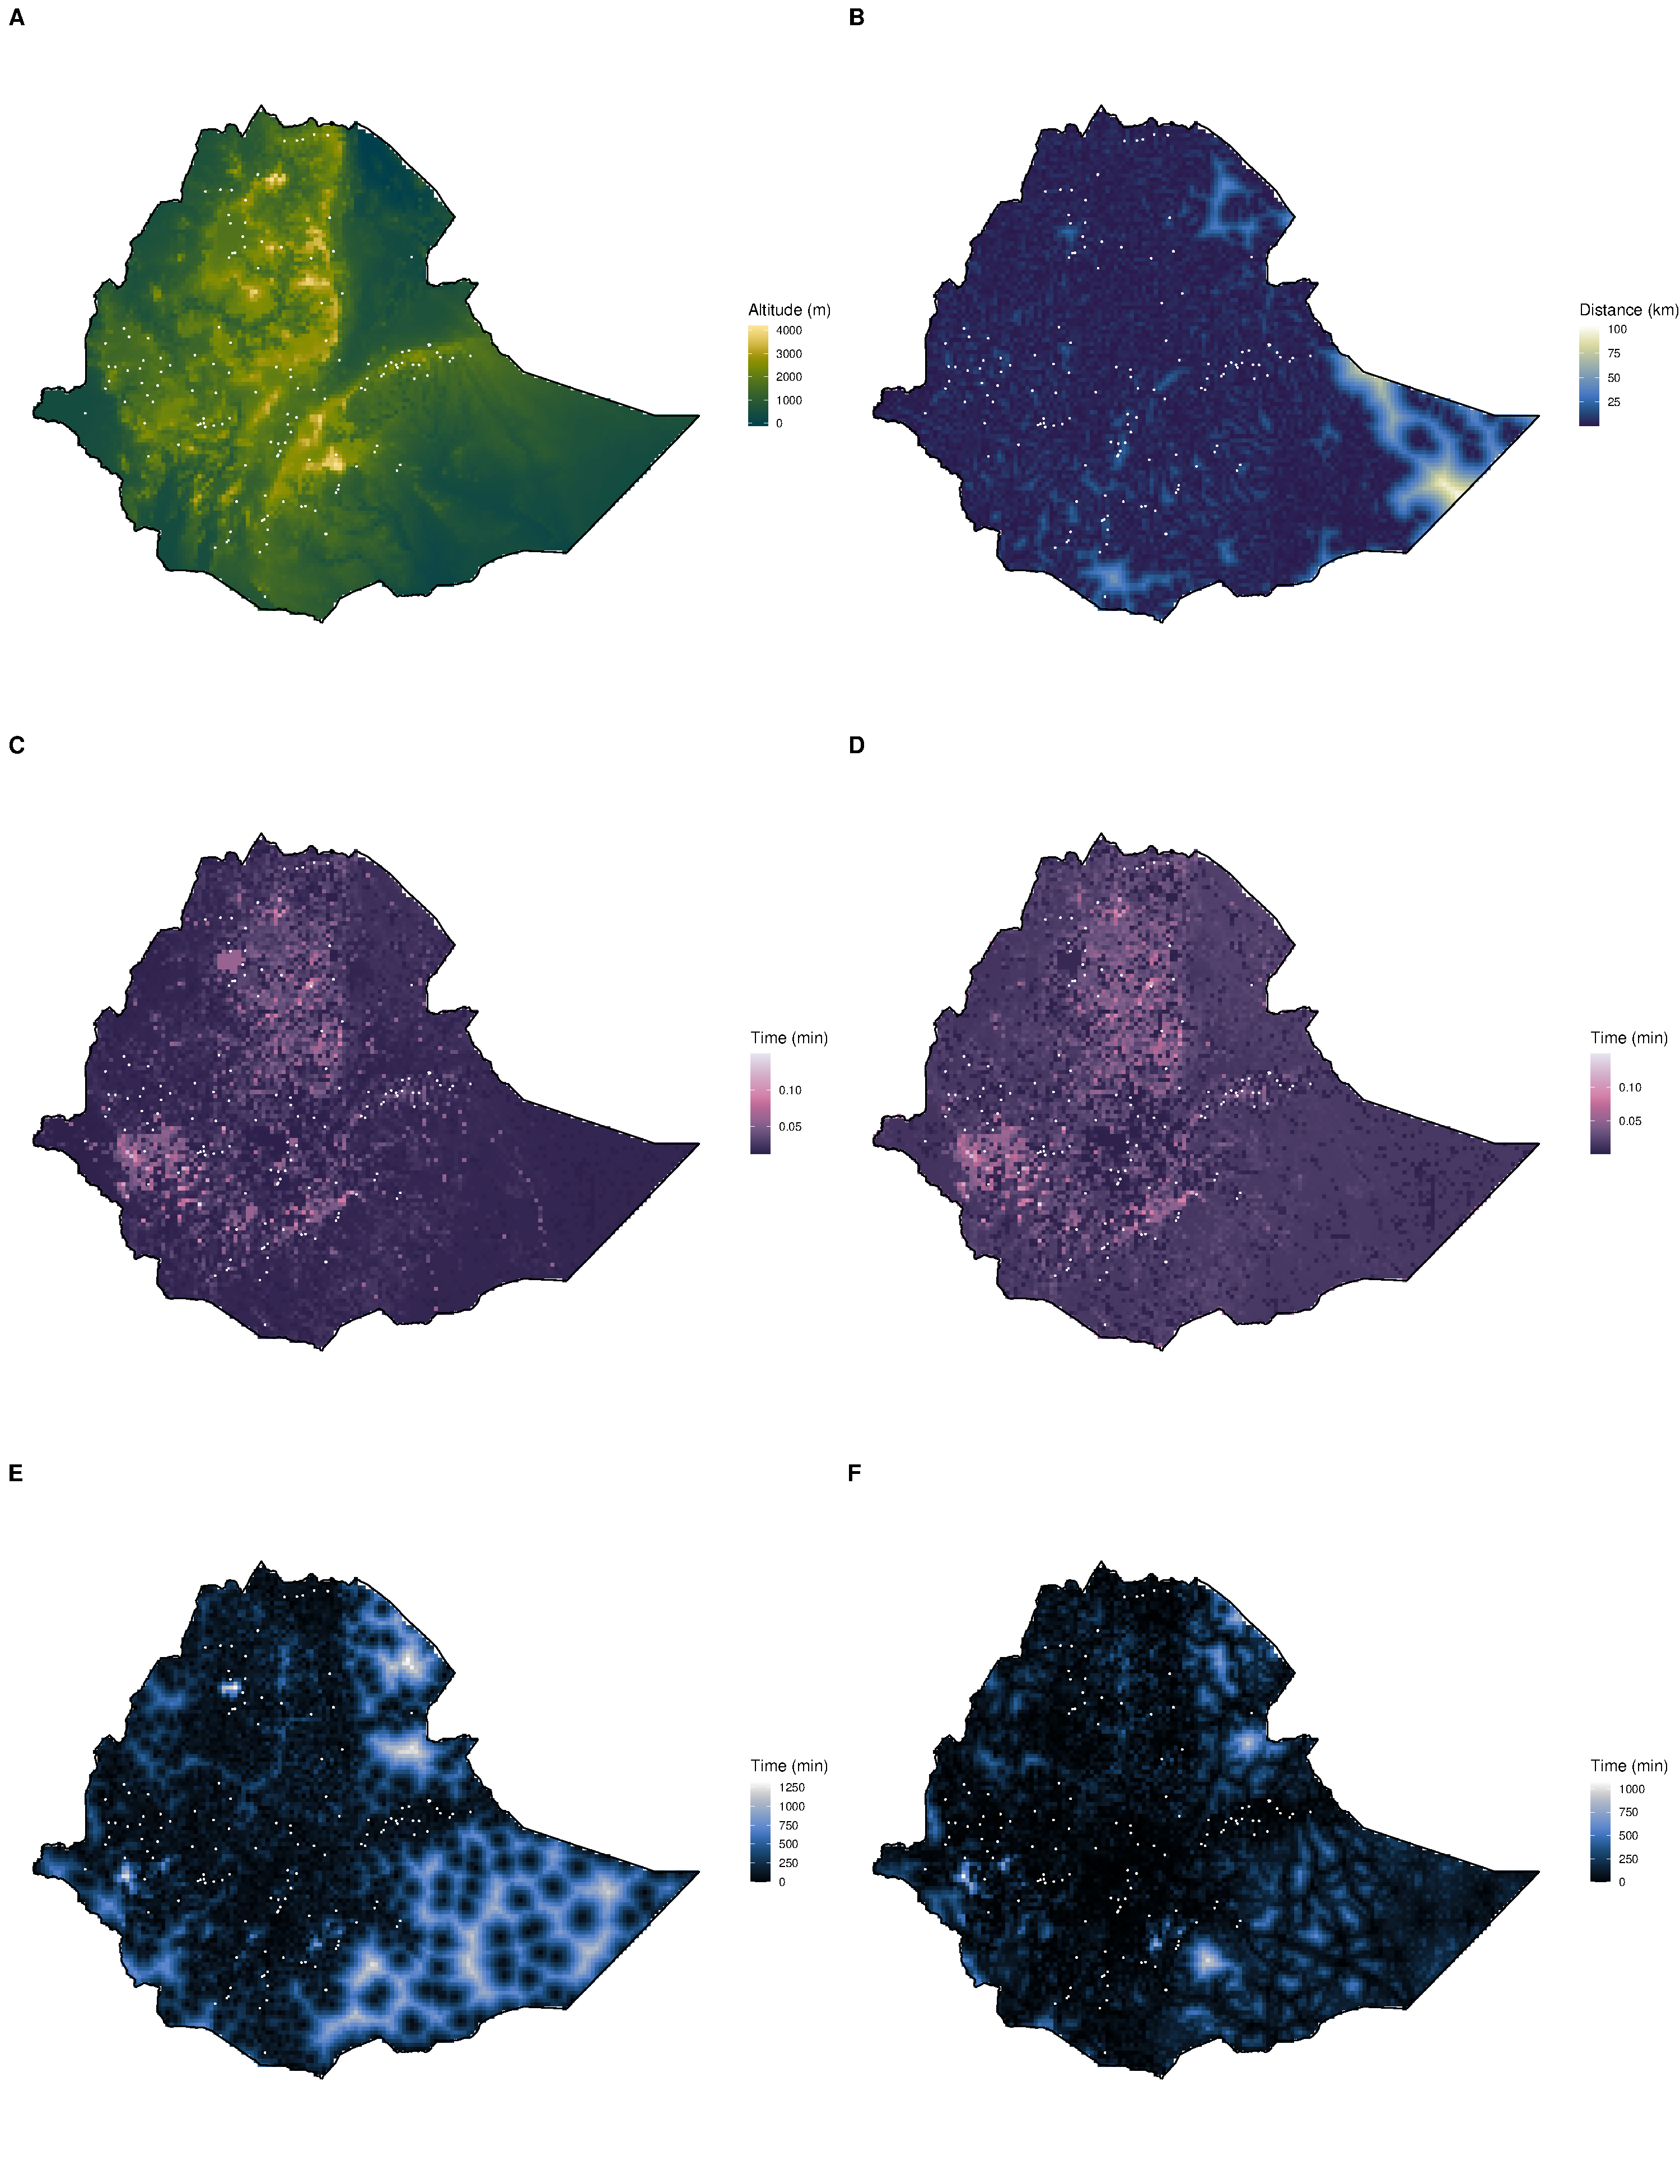
\includegraphics{write_up_files/figure-latex/covariates_figure-1.pdf}
\caption{\textit{Covariate rasters for Ethiopia. A: Altitude, in meters. B: Distance to nearest river, in kilometers. C: Friction surface walking only, in minutes required to travel one meter. D: Friction surface motorized vehicle, same units as C. E: Walking only travel time to nearest healthcare centre, in minutes. F: Motorized vehicle travel time to nearest healthcare centre, in minutes. White dots represent STH data collection points.}}
\end{figure}

\hypertarget{data-analysis}{%
\subsection{Data analysis}\label{data-analysis}}

I started the data analysis by assessing how each covariate was related
to the dependant variable. I created a logit transformation using each
of the three STH species' data, as defined in the equation below. I used
this against each covariate to see how--or if--covariates should be
introduced into the final models.

\[ \text{logit} = \log\left(\frac{y+0.5}{n-y+0.5}\right) \]

Once I had determined the relationship between the covariates and each
of the STH species logit transformation, I proceeded to build binomial
generalised linear mixed-effects models. I created one model for each
species, as defined by the equation below.

\[ \log\left(\frac{p(x_i)}{1-p(x_i)}\right) = d(x_i)^\intercal\beta + Z_i \]

Where:

\begin{itemize}
\tightlist
\item
  \(d(x_i)^\intercal\beta\) holds the intercept and any covariate
  effects at location \(x_i\) included in the model. I selected the
  covariates by assessing associations with the logit transformation
\item
  \(Z_i\) represents the random effects for each location \(x_i\),
  assumed to be normally distributed and independant, identical
  distributions, such that
\end{itemize}

\[ Z_i \sim N(0, \sigma^2)  \]

I assessed if there was overdispersion present by extracting the
variance of the random effects (\(\sigma^2\)). Using a variogram, I
checked if there was residual spatial correlation that remained
unaccounted for by the generalised linear mixed-effects models.

I carried on analysing the data by building a binomial geostatistical
model. This model is defined by the equation below.

\[ \log\left(\frac{p(x_i)}{1-p(x_i)}\right) = d(x_i)^\intercal\beta + S(x_i) + Z_i \]

Where:

\begin{itemize}
\tightlist
\item
  \(d(x_i)^\intercal\beta\) represents the covariate effects at each
  location \(x_i\) and the intercept
\item
  \(S(x_i)\) denotes the spatial Gaussian process, with assumed
  stationarity and isotropy and an exponential correlation function
\item
  \(Z_i\) is the nugget effect, a normally distributed random variable
  representing non-spatial variation, small-scale spatial variation or
  measurement error
\end{itemize}

As this is a binomial geostatistical model, it requires initial guesses
to be given for the unknown parameters. The unknown parameters are:
\(\beta\), the covariate effects at each location \(x_i\) (including the
intercept); \(\sigma^2\), the variance of the spatial Gaussian process;
\(\phi\), the scale of the spatial correlation; and \(\tau^2\), the
variance of the nugget. I used the coefficients of the covariates from a
generalized linear model, which had the same covariates as those
included in the binomial geostatistical model, as the initial guesses
for \(\beta\). I produced the guesses for \(\sigma^2\), \(\phi\) and
\(\tau^2\) by using the empirical variogram and fitting a weighted
least-squares estimate line through it, producing a set a values that
would create this line. I then extracted the values for each of the
parameters from the geostatistical model and used them as guesses for
the same model. I repeated this until the values of the parameters
stabilised.

I performed the inference explained above using Markov Chain Monte Carlo
(MCMC) methods. I ran 10,000 simulations, discarding the first 2,000
results and only keeping every 8\^{}th result thereafter. This resulted
in 1,000 samples per location.

\hypertarget{prediction}{%
\subsection{Prediction}\label{prediction}}

To create a predicted prevalence raster for Ethiopia, I made a grid of
points across the entire country, at a resolution of 10 km. I extracted
the values for each of the covariates at each of these points and saved
them as a data frame. I used this data frame to predict the prevalence
of each of the STH species at every grid point, using the same MCMC
methods described previously.

To create a raster of the prevalence of at least one STH species, I
extracted the MCMC samples for each of the species. I then used this to,
firstly, estimate the ``anti-prevalence'' of each species and, secondly,
combine these to estimate the prevalence of at least one species. This
is described in the equation below.

\[ P(S_1 \vee S_2 \vee S_3) = 1 - P(\bar{S_1} \wedge \bar{S_2} \wedge \bar{S_3}) \]

I used these samples of at least one species to create two probability
rasters: one showing the probability of exceeding 50\% prevalence and a
second showing the probability of having between 20\% and 50\%
prevalence. I combined these rasters to create maps to show what areas
needed different strategies, at three different confidence levels: 90\%
confidence, 75\% confidence and 60\% confidence. The strategies referred
to the recommendations set out by the WHO, where MDAs should happen
twice a year for areas with over 50\% prevalence of STH, once a year for
areas with prevalence between 20\% and 50\% and strategies should move
to a case-by-case basis in areas where prevalence was below 20\%. I also
created a fourth category to indicate areas where confidence was too low
and would therefore need further investigations.

\hypertarget{results}{%
\section{Results}\label{results}}

\hypertarget{espen-data}{%
\subsection{ESPEN data}\label{espen-data}}

There were a total of 146 unique data collection locations across
Ethiopia (Figure 2). The data collection occurred across a number of
years, at varying rates, as described in Table 1. Due to lack of
multiple rasters representing the change in time, this temporal change
was not accounted for in any further analyses.

\begin{figure}
\centering
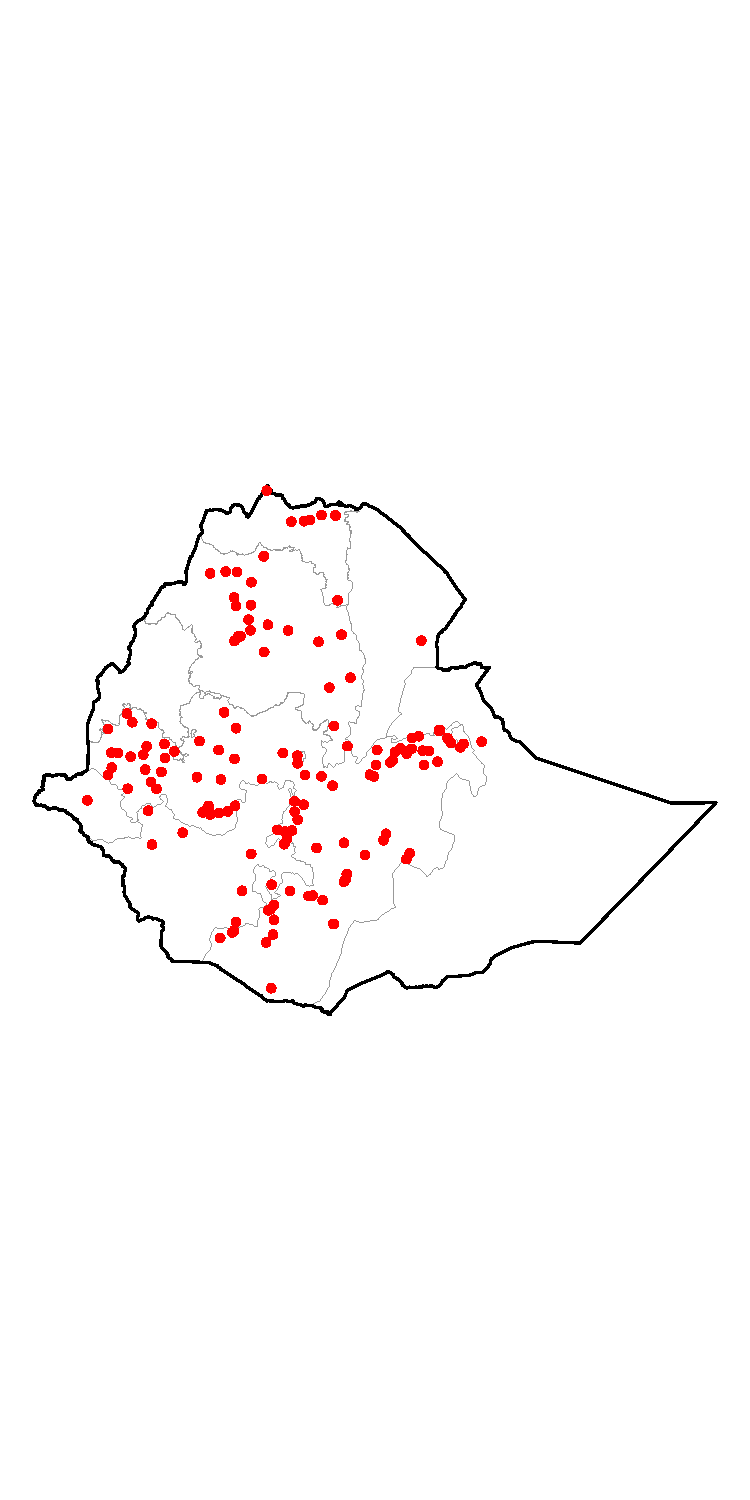
\includegraphics{write_up_files/figure-latex/STH_locations-1.pdf}
\caption{\textit{STH data collection locations.}}
\end{figure}

\newpage

\begin{longtable}[]{@{}rr@{}}
\caption{Number of STH surveys performed by year.}\tabularnewline
\toprule
Year & Number of surveys \\
\midrule
\endfirsthead
\toprule
Year & Number of surveys \\
\midrule
\endhead
2001 & 1 \\
2003 & 1 \\
2005 & 60 \\
2008 & 1 \\
2009 & 102 \\
2010 & 2 \\
2011 & 1 \\
2012 & 3 \\
2013 & 7 \\
2014 & 1 \\
2015 & 2 \\
\bottomrule
\end{longtable}

\hypertarget{hookworms}{%
\subsection{Hookworms}\label{hookworms}}

I performed a logit transformation on the hookworm data to determine the
association with each of the covariates (Figure 3).

\begin{figure}
\centering
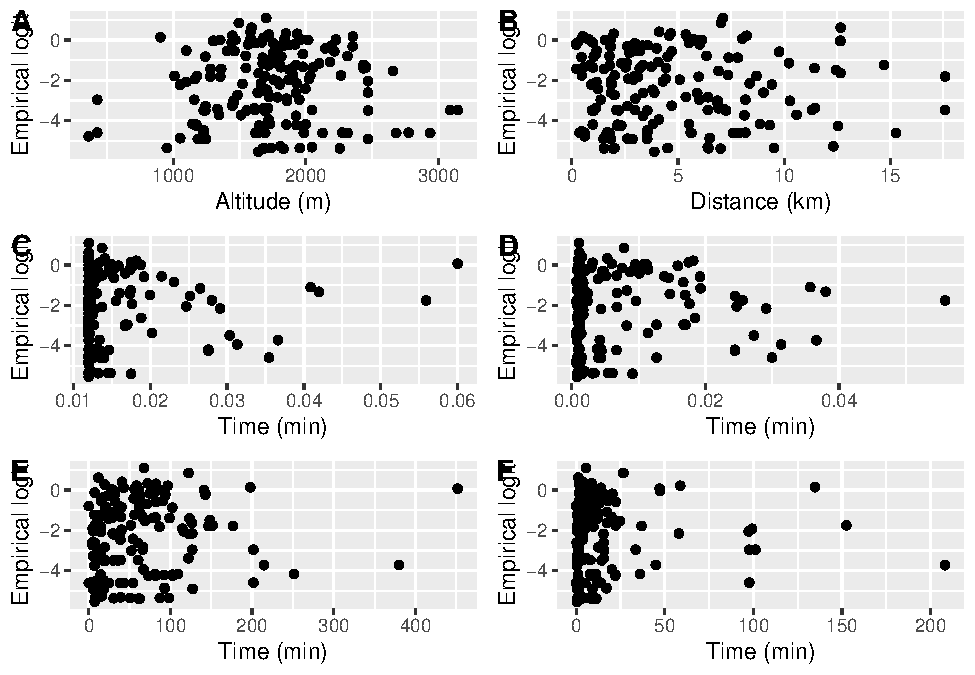
\includegraphics{write_up_files/figure-latex/HK_e.logit-1.pdf}
\caption{\textit{Covariates against empirical logit transformation of hookworm data. A: Altitude, in meters. B: Distance to nearest river, in kilometers. C: Friction surface walking only, in minutes required to travel one meter. D: Friction surface motorized vehicle, same units as C. E: Walking only travel time to nearest healthcare centre, in minutes. F: Motorized vehicle travel time to nearest healthcare centre, in minutes.}}
\end{figure}

Focusing on altitude, most of the data points are located in the middle
of the range, with a few points on either side. There does appear to be
a linear relationship present, with the empirical logit increasing as
altitude increases. With distance to river, there is a high density of
points located in the lower end of the range. The friction variables and
the travel variables show very similar relationships. Most of the data
points are located on the lower end of the scales. The walking travel
time to nearest healthcare centre has the lowest density, with the
points more spread out across the range.

Informed by these plots, I decided to include altitude, distance to
river and walking travel time to nearest health care centre in further
models. I only included one of the friction and travel variables due to
risks of introducing multi-collinearity.

I used these variables, without performing any transformations on them,
to build a binomial generalised linear mixed-effects model, as defined
in the methods section. The variance of the random effects was 3.59,
showing evidence of overdispersion. The variogram for this model also
showed residual spatial correlation (Figure 4).

\begin{figure}
\centering
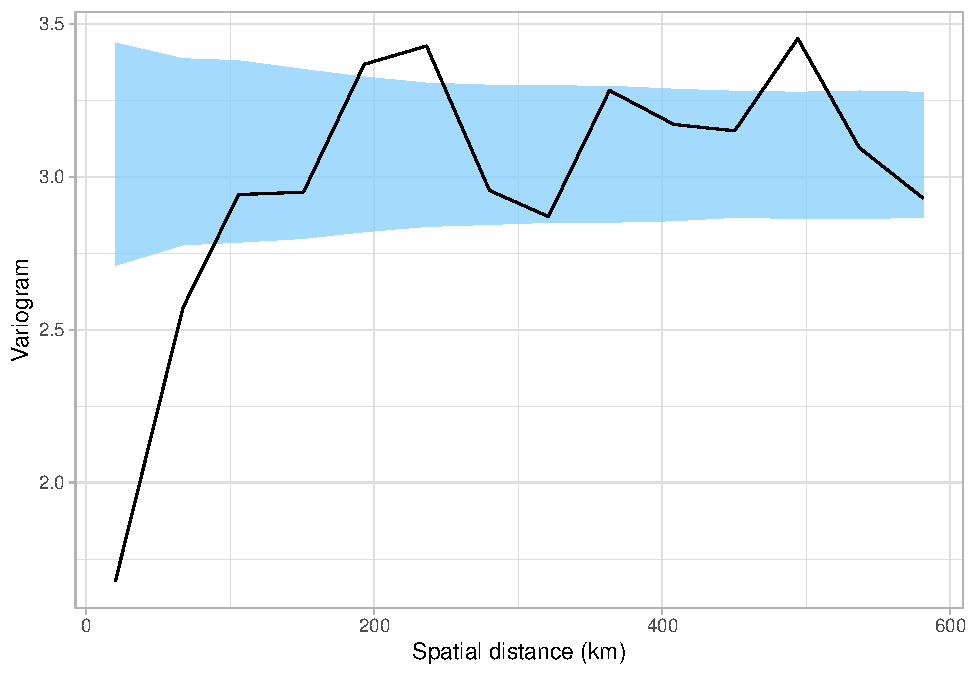
\includegraphics{write_up_files/figure-latex/HK.variogram_2-1.pdf}
\caption{\textit{Variogram of Hookworm data. Plot shows evidence of residual spatial correlation that remains unaccounted for by the generalised linear mixed-effects model.}}
\end{figure}

I followed by building a binomial geostatistical model, as described in
the methods section. I performed four rounds of using guesses for the
model parameters before arriving to a final model. The final parameters
are described in Table 2.

\begin{longtable}[]{@{}lrr@{}}
\caption{Estimated parameters from binomial geostatistical model -
Hookworms}\tabularnewline
\toprule
& Estimate & StdErr \\
\midrule
\endfirsthead
\toprule
& Estimate & StdErr \\
\midrule
\endhead
\(\sigma^2\) & 3.126 & 0.091 \\
\(\phi\) & 76.982 & 0.006 \\
\(\tau^2\) & 1.154 & 0.445 \\
\bottomrule
\end{longtable}

Using this model, I created three rasters: one showing the predicted
prevalence of hookworms across Ethiopia, one showing the probability of
having between 20\% and 50\% prevalence and the final one showing the
probability of exceeding 50\% prevalence (Figure 5).

\begin{figure}
\centering
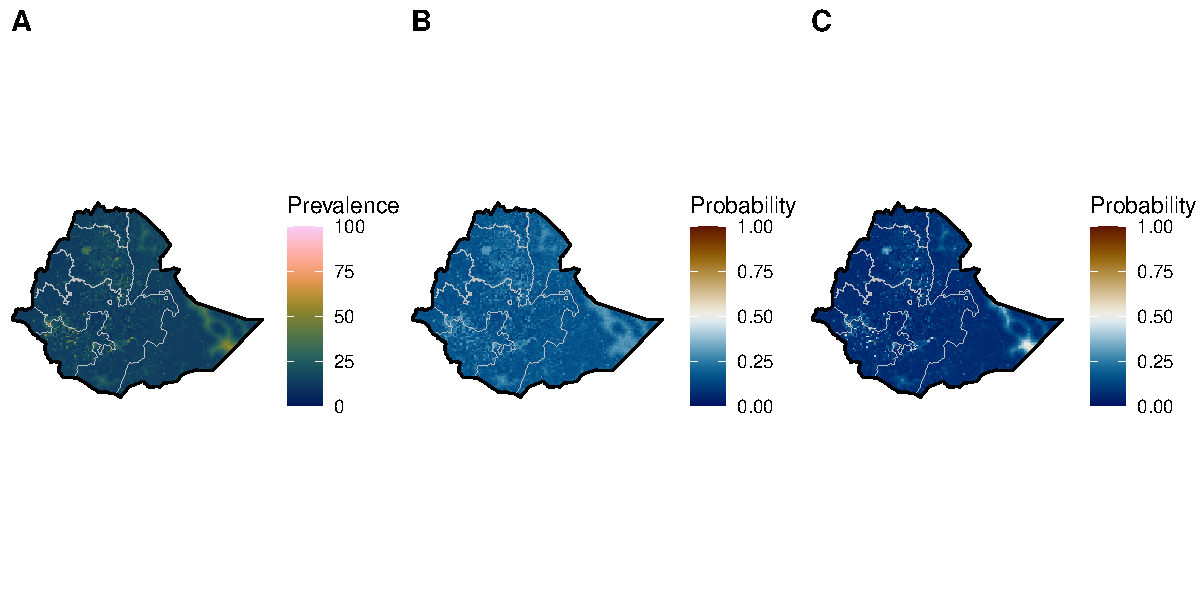
\includegraphics{write_up_files/figure-latex/HK.prediction.rasters-1.pdf}
\caption{\emph{Rasters for Hookworm estimates. A: Predicted prevalence.
B: Probability of having prevalence between 20\% and 50\%. C:
Probability of exceeding 50\% prevalence.}}
\end{figure}

The predicted prevalence shows a pocket of high prevalence of hookworm
in the eastern region of Ethiopia. This area does overlap with a high
probability of exceeding 50\% prevalence. However, there is low
probability of having between 20\% and 50\% prevalence across the entire
country.

\newpage

\hypertarget{ascaris-lumbricoides}{%
\subsection{\texorpdfstring{\emph{Ascaris
lumbricoides}}{Ascaris lumbricoides}}\label{ascaris-lumbricoides}}

The associations between each covariate and the logit transformation for
the Ascaris lumbricoides data is plotted in Figure 6.

\begin{figure}
\centering
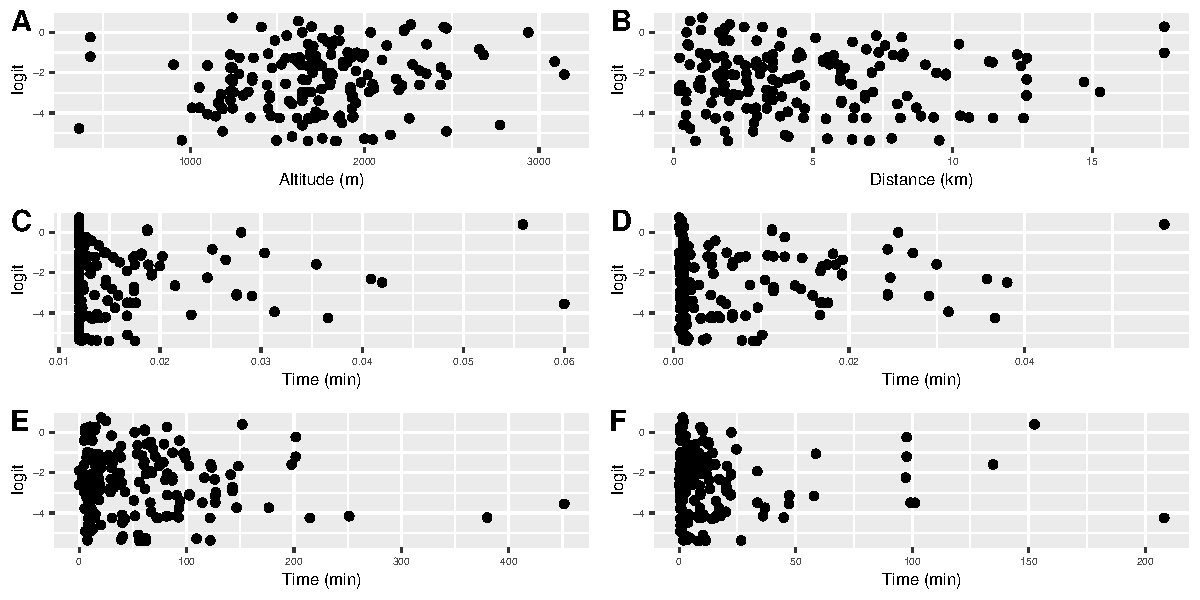
\includegraphics{write_up_files/figure-latex/Asc_e.logit-1.pdf}
\caption{\textit{Covariates against empirical logit transformation of Ascaris lumbricoides data. A: Altitude, in meters. B: Distance to nearest river, in kilometers. C: Friction surface walking only, in minutes required to travel one meter. D: Friction surface motorized vehicle, same units as C. E: Walking only travel time to nearest healthcare centre, in minutes. F: Motorized vehicle travel time to nearest healthcare centre, in minutes.}}
\end{figure}

All the associations are very similar to those seen for the hookworm
logit transformation. Both altitude and distance to nearest river show
less concentration of data points across the ranges, but this does not
seem to affect the associations with the logit data. As with hookworms,
the travel and friction data show a high density of data points on the
lower end of the range. I decided to include the same covariates as for
hookworm: altitude, distance to nearest river and walking travel time to
closest healthcare centre.

The binomial generalised linear mixed-effects model showed evidence of
overdispersion, as the variance of the random effects was 2.087. The
variogram for this model also showed the presence of residual spatial
correlation (Figure 7).

\begin{figure}
\centering
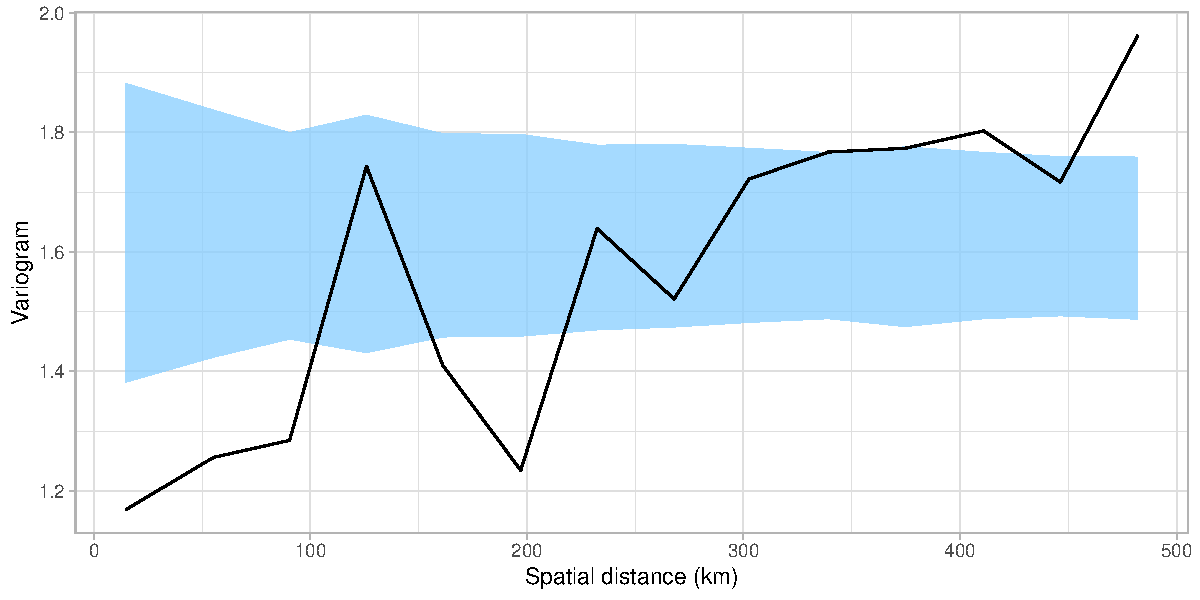
\includegraphics{write_up_files/figure-latex/Asc.variogram_2-1.pdf}
\caption{\textit{Variogram of Ascaris lumbricoides data. Plot shows evidence of residual spatial correlation that remains unaccounted for by the generalised linear mixed-effects model.}}
\end{figure}

I performed four rounds of parameter guessing before reaching a final
binomial geostatistical model. These are described in Table 3.

\begin{longtable}[]{@{}lrr@{}}
\caption{Estimated parameters from binomial geostatistical model -
Ascaris lumbricoides}\tabularnewline
\toprule
& Estimate & StdErr \\
\midrule
\endfirsthead
\toprule
& Estimate & StdErr \\
\midrule
\endhead
\(\sigma^2\) & 1.575 & 0.271 \\
\(\phi\) & 172.627 & 0.003 \\
\(\tau^2\) & 0.995 & 0.753 \\
\bottomrule
\end{longtable}

I used this model to create the same three rasters as I did for
hookworms: predicted prevalence, probability of having between 20\% and
50\% prevalence and probability of exceeding 50\% prevalence (Figure 8).

\begin{figure}
\centering
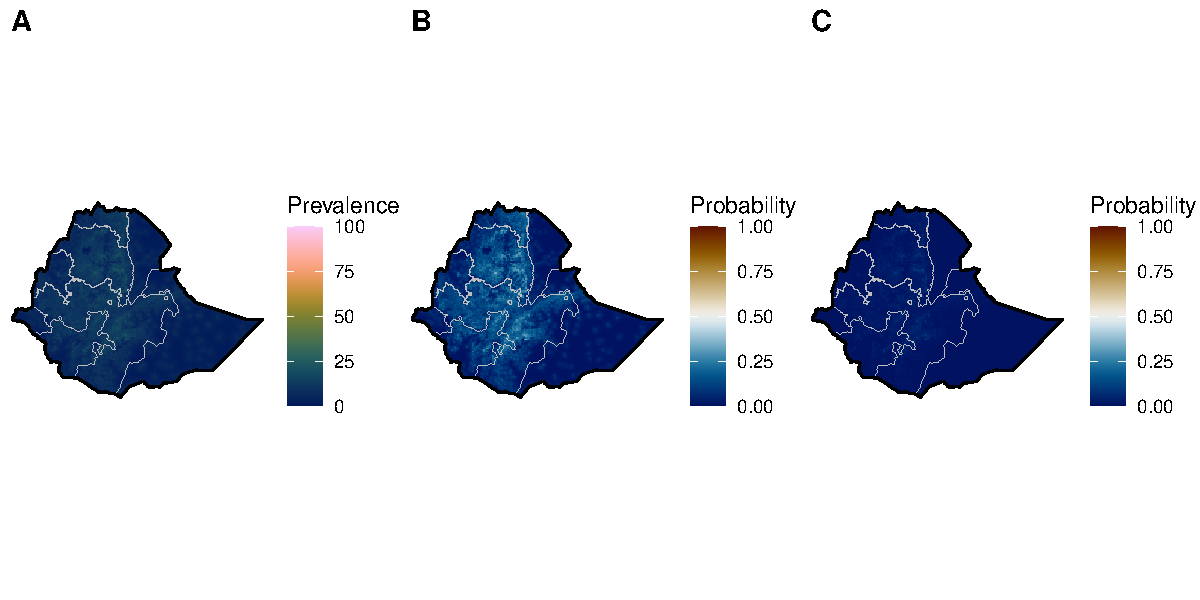
\includegraphics{write_up_files/figure-latex/Asc.prediction.rasters-1.pdf}
\caption{\emph{Rasters for Ascaris lumbricoides estimates. A: Predicted
prevalence. B: Probability of having prevalence between 20\% and 50\%.
C: Probability of exceeding 50\% prevalence.}}
\end{figure}

These maps show that the prevalence for Ascaris lumbricoides across
Ethiopia is very low.

\newpage

\hypertarget{trichuris-trichuria}{%
\subsection{\texorpdfstring{\emph{Trichuris
trichuria}}{Trichuris trichuria}}\label{trichuris-trichuria}}

I plotted the logit transformed Trichuris trichuria data against each of
the covariates (Figure 9).

\begin{figure}
\centering
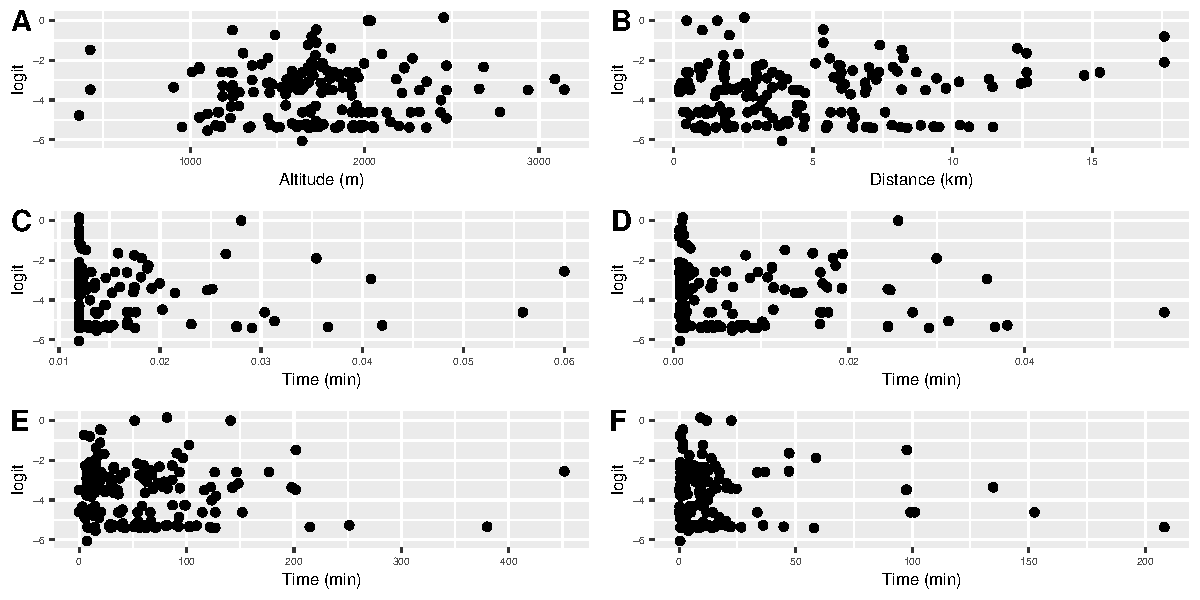
\includegraphics{write_up_files/figure-latex/TT_e.logit-1.pdf}
\caption{\textit{Covariates against empirical logit transformation of Trichuris trichuria data. A: Altitude, in meters. B: Distance to nearest river, in kilometers. C: Friction surface walking only, in minutes required to travel one meter. D: Friction surface motorized vehicle, same units as C. E: Walking only travel time to nearest healthcare centre, in minutes. F: Motorized vehicle travel time to nearest healthcare centre, in minutes.}}
\end{figure}

The only notable difference of the Trichuris trichuria logit data is
that when plotting it against the distance to river it seems to be more
spread out than the data points for hookworms and \emph{Ascaris
lumbricoides}. All other associations are very similar. Therefore, I
used the same covariates as I did in models for hookworms and for
\emph{Ascaris lumbricoides}.

The binomial generalised linear mixed-effects model also showed evidence
of overdispersion for \emph{Trichuris trichuria}, as the variance of the
random effects was 2.269. The variogram showed evidence of residual
spatial correlation (figure 10).

\begin{figure}
\centering
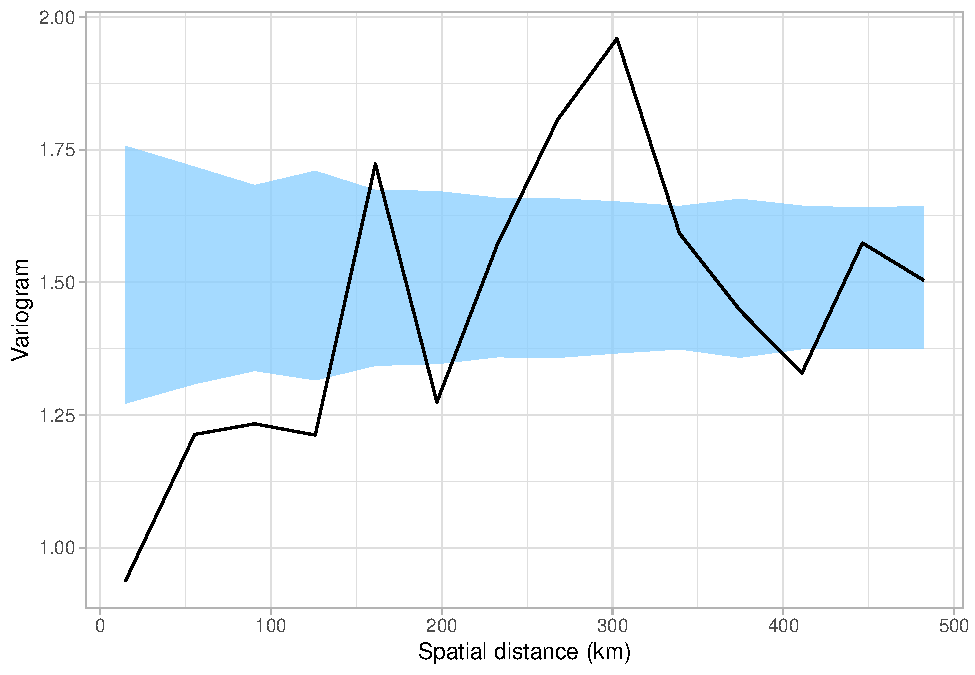
\includegraphics{write_up_files/figure-latex/TT.variogram_2-1.pdf}
\caption{\textit{Variogram of Ascaris lumbricoides data. Plot shows evidence of residual spatial correlation that remains unaccounted for by the generalised linear mixed-effects model.}}
\end{figure}

I ran the parameter guesses six times until I reached a final model. The
parameters are described in Table 5. I predicted the prevalence and the
probability rasters for Trichuris trichuria using this model (Figure
11).

\begin{longtable}[]{@{}lrr@{}}
\caption{Estimated parameters from binomial geostatistical model -
Trichuris trichuria}\tabularnewline
\toprule
& Estimate & StdErr \\
\midrule
\endfirsthead
\toprule
& Estimate & StdErr \\
\midrule
\endhead
\(\sigma^2\) & 1.804 & 0.178 \\
\(\phi\) & 75.202 & 0.006 \\
\(\tau^2\) & 0.661 & 0.865 \\
\bottomrule
\end{longtable}

\begin{figure}
\centering
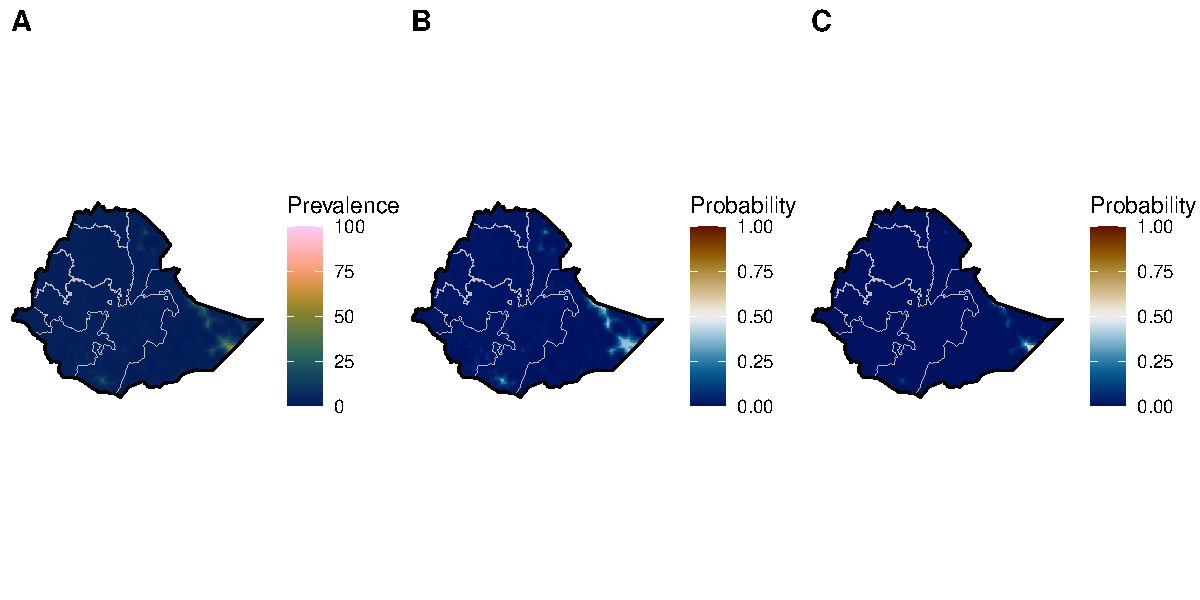
\includegraphics{write_up_files/figure-latex/TT.prediction.rasters-1.pdf}
\caption{\emph{Rasters for Trichuris trichuria estimates. A: Predicted
prevalence. B: Probability of having prevalence between 20\% and 50\%.
C: Probability of exceeding 50\% prevalence.}}
\end{figure}

These maps show that, overall, there is very low prevalence of
\emph{Trichuris trichuria} across Ethiopia. The only exception is a
small area in the eastern region of Ethiopia, where prevalence appears
to be extremely high.

\newpage

\hypertarget{any-sth-species}{%
\subsection{Any STH species}\label{any-sth-species}}

As described in the methods section, I combined the estimated
prevalences of the three STH species to create an estimated prevalence
of any STH species. I used this estimate to create 3 rasters: one
showing the estimated prevalence, one showing the probability of having
between 20\% and 50\% prevalence and a third showing the probability of
exceeding 50\% prevalence (Figure 12).

\begin{figure}
\centering
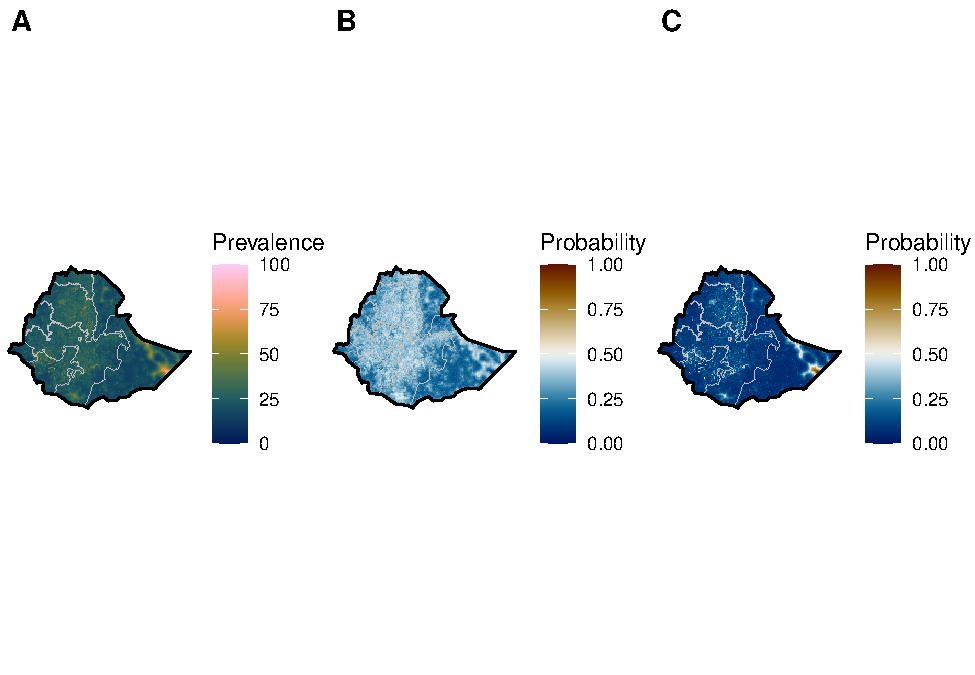
\includegraphics{write_up_files/figure-latex/any.sth.prediction.rasters-1.pdf}
\caption{\emph{Rasters for any STH species' estimates. A: Predicted
prevalence. B: Probability of having prevalence between 20\% and 50\%.
C: Probability of exceeding 50\% prevalence.}}
\end{figure}

These maps show that, as described above, there is an area in the
eastern region of Ethiopia that does have high prevalence for any STH
species.

I combined these estimates to create a discrete raster, identifying what
strategy should be used in which area. I created these with three levels
of confidence (Figure 13).

\begin{figure}
\centering
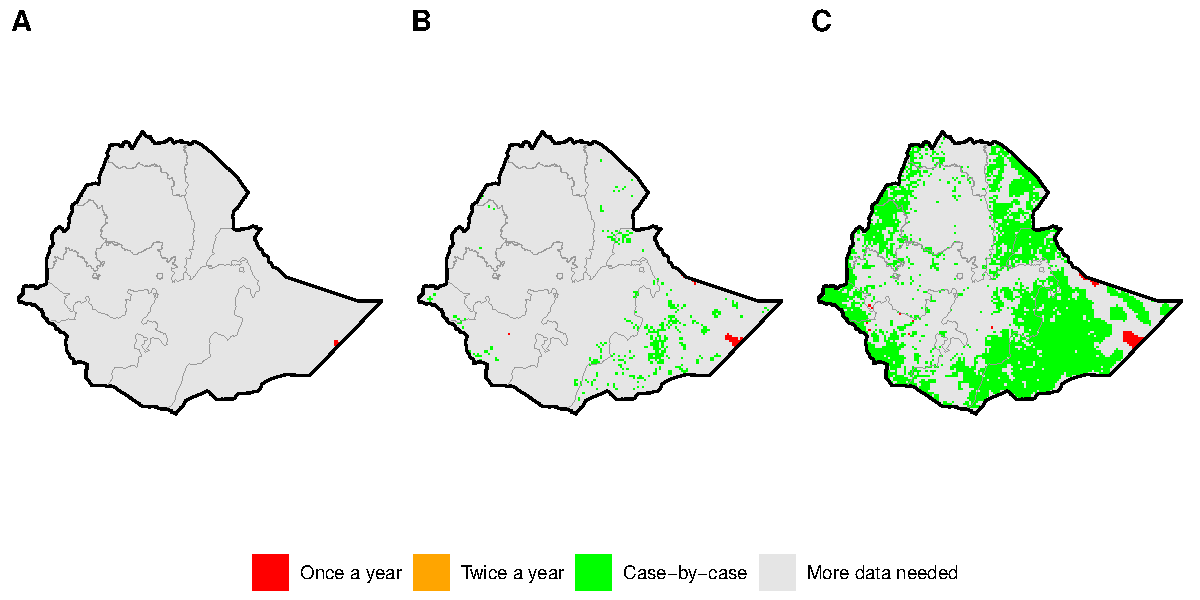
\includegraphics{write_up_files/figure-latex/discrete.rasters-1.pdf}
\caption{\emph{STH control strategies to use for each area, by
confidence level. A: 90\% confidence, B: 75\% confidence C: 60\%
confidence.}}
\end{figure}

These maps show that, depending on the level of confidence, different
areas would require different interventions.

\newpage

\hypertarget{conclusion}{%
\section{Conclusion}\label{conclusion}}

In this report, I used geostatistical methods to produce an estimate of
STH prevalence across Ethiopia. I used this estimate to create maps
identifying which areas required which control strategy, depending on
the level of confidence needed.

These maps showed that, overall, more data would be better to create a
more informative estimate. However, given that getting more and better
quality data is not always feasible, considering other options is
important. My choice of covariates might have been inadequate, given the
level of uncertainty in the final plots. Including covariates which
represented temporal changes, as well as spatial ones, could have
produced more accurate and dynamic maps. There is also a large area in
the eastern region of Ethiopia where no data collection took place.
Whilst the predictions for this area should be interpreted with caution,
this area represents a good example of the usefulness of geostatistical
models. By using spatial data that is openly available, I can predict
the prevalence in an area which might not be easy to survey. It would be
essential to understand the reasoning behind the lack of data, as this
could affect how the predictions are interpreted. If there is a specific
difference between the people living here and those in areas where data
collection took place--for example, different cultural practices
resulting in different risks of STH--this could result in invalid
predictions. This highlights the necessity of having open dialogue
across disciplines.

This report also shows the importance of working alongside policy makes
in making decisions. Changing the confidence level of the final data can
have different outcomes. Ultimately, this decision is set by policy
makers and should be done in conversation with other professionals,
including health economists and anthropologists.

\hypertarget{references}{%
\section*{References}\label{references}}
\addcontentsline{toc}{section}{References}

\hypertarget{refs}{}
\begin{CSLReferences}{0}{0}
\leavevmode\vadjust pre{\hypertarget{ref-worldhealthorganizationEliminatingSoiltransmittedHelminthiases2012}{}}%
1. Organization WH. Eliminating soil-transmitted helminthiases as a
public health problem in children. {Progress} report 2001-2010 and
strategic plan 2011-2020. {World Health Organization}; 2012.

\leavevmode\vadjust pre{\hypertarget{ref-sartoriusPrevalenceIntensitySoiltransmitted2021}{}}%
2. Sartorius B, Cano J, Simpson H, Tusting LS, Marczak LB, Miller-Petrie
MK, et al.
\href{https://doi.org/10.1016/S2214-109X(20)30398-3}{Prevalence and
intensity of soil-transmitted helminth infections of children in
sub-{Saharan Africa}, 2000\textendash 18: A geospatial analysis}. The
Lancet Global Health. {Elsevier}; 2021;9:e52--60.

\leavevmode\vadjust pre{\hypertarget{ref-aemiroPrevalenceSoilTransmittedHelminthes2022}{}}%
3. Aemiro A, Menkir S, Tegen D, Tola G.
\href{https://doi.org/10.1177/11786337211055437}{Prevalence of
{Soil-Transmitted Helminthes} and {Associated Risk Factors Among People}
of {Ethiopia}: {A Systematic Review} and {Meta-Analysis}}. Infectious
Diseases: Research and Treatment. {SAGE Publications Ltd STM};
2022;15:11786337211055437.

\leavevmode\vadjust pre{\hypertarget{ref-ESPENExpandedSpecial}{}}%
4. {ESPEN} \textbar{} {Expanded Special Project} for {Elimination
Neglected Tropical Diseases}. https://espen.afro.who.int/;

\leavevmode\vadjust pre{\hypertarget{ref-alelignSoilTransmittedHelminthInfections2015}{}}%
5. Alelign T, Degarege A, Erko B.
\href{https://doi.org/10.1155/2015/641602}{Soil-{Transmitted Helminth
Infections} and {Associated Risk Factors} among {Schoolchildren} in
{Durbete Town}, {Northwestern Ethiopia}}. Journal of Parasitology
Research. {Hindawi}; 2015;2015:e641602.

\leavevmode\vadjust pre{\hypertarget{ref-anegagrieEnvironmentalCharacteristicsHousehold2021}{}}%
6. Anegagrie M, Lanfri S, Aramendia AA, Scavuzzo CM, Herrador Z, Benito
A, et al.
\href{https://doi.org/10.1371/journal.pntd.0009466}{Environmental
characteristics around the household and their association with hookworm
infection in rural communities from {Bahir Dar}, {Amhara Region},
{Ethiopia}}. PLOS Neglected Tropical Diseases. {Public Library of
Science}; 2021;15:e0009466.

\leavevmode\vadjust pre{\hypertarget{ref-eyayuPrevalenceIntensityInfection2022}{}}%
7. Eyayu T, Yimer G, Workineh L, Tiruneh T, Sema M, Legese B, et al.
\href{https://doi.org/10.1371/journal.pone.0266333}{Prevalence,
intensity of infection and associated risk factors of soil-transmitted
helminth infections among school children at {Tachgayint} woreda,
{Northcentral Ethiopia}}. PLOS ONE. {Public Library of Science};
2022;17:e0266333.

\leavevmode\vadjust pre{\hypertarget{ref-DIVAGISFreeSimple}{}}%
8. {DIVA-GIS} \textbar{} free, simple \& effective.
https://www.diva-gis.org/;

\leavevmode\vadjust pre{\hypertarget{ref-MalariaAtlasProject}{}}%
9. The {Malaria Atlas Project}. MAP. https://malariaatlas.org/;

\end{CSLReferences}

\end{document}
